\documentclass{article}

\usepackage[most]{tcolorbox}
\usepackage{physics}
\usepackage{graphicx}
\usepackage{float}
\usepackage{amsmath}
\usepackage{amssymb}


\usepackage[utf8]{inputenc}
\usepackage[a4paper, margin=1in]{geometry} % Controla los márgenes
\usepackage{titling}

\title{Clase Agujeros Negros }
\author{Manuel Garcia.}
\date{\today}

\renewcommand{\maketitlehooka}{%
  \centering
  \vspace*{0.05cm} % Espacio vertical antes del título
}

\renewcommand{\maketitlehookd}{%
  \vspace*{2cm} % Espacio vertical después de la fecha
}

\newcommand{\caja}[3]{%
  \begin{tcolorbox}[colback=#1!5!white,colframe=#1!25!black,title=#2]
    #3
  \end{tcolorbox}%
}

\begin{document}
\maketitle

\section{}
Ecuación de Klein-Gordon 
\begin{gather*}
  (\Box - m^2) \phi(x) = 0 
\end{gather*}
Solución 
\begin{gather*}
   \phi_\Omega (t,\vec x) = \phi_\Omega (r) Y _{lm } (\theta,\phi) \frac{1}{\sqrt{2 \left|\omega \right|} } e ^ {- i \omega t }
\end{gather*}

\hfill 

\hfill 

\hfill 

\begin{figure}[H]
  \begin{center}
    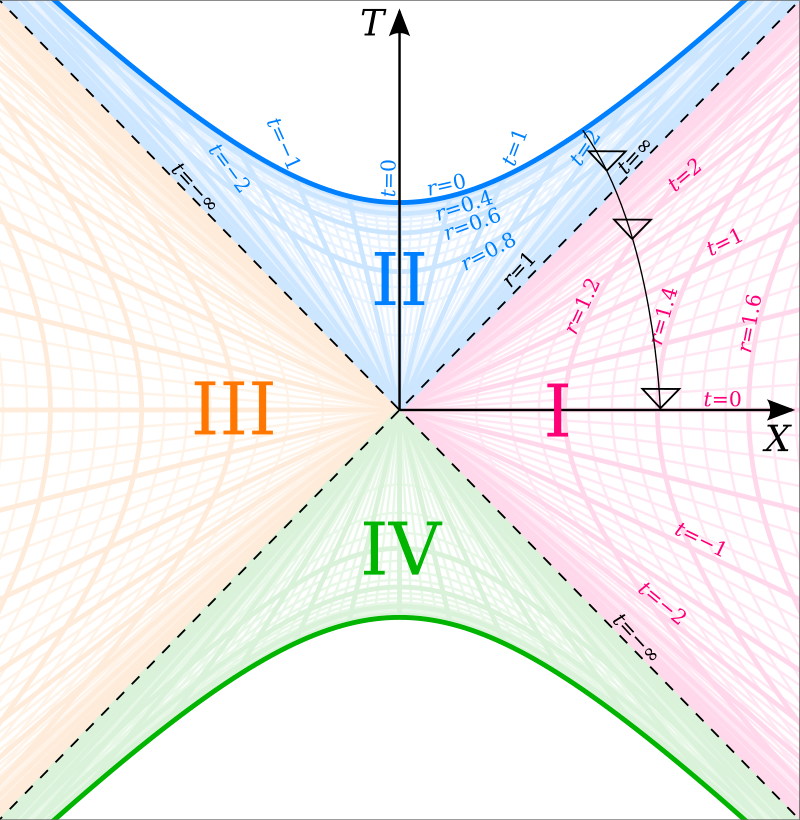
\includegraphics[width=0.35\textwidth]{kruskal.png}
  \end{center}
\end{figure}



Considérese los t-modos para I 
\begin{gather*}
  \phi _\Omega = \phi_\Omega (\vec x) \frac{1}{\sqrt{2 \left|\omega\right|} } e ^ {- i \omega t } 
\end{gather*}

Sean los Killing-Boulware (KB-modos) para I y III
\begin{gather*}
  \phi_\Omega ^ {(\epsilon)}(x) = \phi_\Omega (\vec x, t) \Theta_\epsilon (x)
  \qquad \qquad \text{Con } \epsilon= \pm 1 \text{ y } \Theta_\epsilon(x) \text{ la función unitaria }   \\
  \Theta_\epsilon(x) := \frac{1}{2} \{\Theta(-\epsilon u ) + \Theta(\epsilon v )  \} \qquad \text{En el E-T de Kruskal }
\end{gather*}

\caja{black}{Ejemplo }{
  Calcular $ \Theta _+ $ para I 
  \begin{gather*}
    \Theta_+(x) = \frac{1}{2} \{\Theta(-U) + \Theta(V )\} 
  \end{gather*}
  Como es en la region I se tiene que $ \Theta(-U ) = +1  $ y $ \Theta(V ) = 1  $
  \begin{gather*}
    \Theta_+ (x) = 1 
  \end{gather*}
}

\caja{red}{Ejercicio }{
  \begin{itemize}
    \item 
      Calcular $ \Theta_-  $ para I 
      \begin{gather*}
        \Theta_-(x) = \frac{1}{2} \{\Theta(U) + \Theta(-V )\} 
      \end{gather*}
      En la region I se tiene que $ \Theta(U) = 0  $ y $ \Theta(-V) = 0  $
      \begin{gather*}
        \Theta_-(x) = 0 
      \end{gather*}
    
    \item 
      Calcular $ \Theta_+  $ para III 
      \begin{gather*}
        \Theta_+(x) = \frac{1}{2} \{\Theta(-U) + \Theta(V )\} 
      \end{gather*}
      En la region III se tiene que $ \Theta(-U) = 0  $ y $ \Theta(V) = 0  $, por lo tanto $ \Theta_+(x) = 0  $\\
    
    \item 
      Calcular $ \Theta_-  $ para III 
      \begin{gather*}
        \Theta_-(x) = \frac{1}{2} \{\Theta(U) + \Theta(-V )\} 
      \end{gather*}
      En la region III se tiene que $ \Theta(U) = +1  $ y $ \Theta(-V) = +1  $, por lo tanto $ \Theta_-(x) = 1  $
  \end{itemize}
}


\caja{green}{Ejercicios para la casa}{
  \begin{enumerate}
    \item probar que 
      \begin{enumerate}
        \item $ \Theta_\epsilon + \Theta _{-\epsilon}  = 1  $
        
        \item $ \Theta_\epsilon - \Theta _{-\epsilon }  = \frac{1}{2}\epsilon\{\epsilon(V) - \epsilon(U) \} \qquad $ donde $\quad \epsilon(V) \equiv sign (V) $, $ \ \epsilon(U) \equiv sign(U) $
      \end{enumerate}
  \end{enumerate}
}


\end{document}
